\documentclass[crop, tikz]{standalone}

\usepackage{tikz}
\usepackage{amsmath}
\usepackage{amssymb}
\usepackage[mode=buildnew]{standalone}

\usepackage{xcolor}


\usetikzlibrary{positioning}
\usetikzlibrary{calc}
\usetikzlibrary{fit}
%\usepackage{nicematrix}

\tikzset{set/.style={draw,circle,inner sep=0pt,align=center}}

\definecolor{mred}{RGB}{214,39,40}
\definecolor{mgreen}{RGB}{44,160,44}
\definecolor{mblue}{RGB}{31,119,180}


\begin{document}

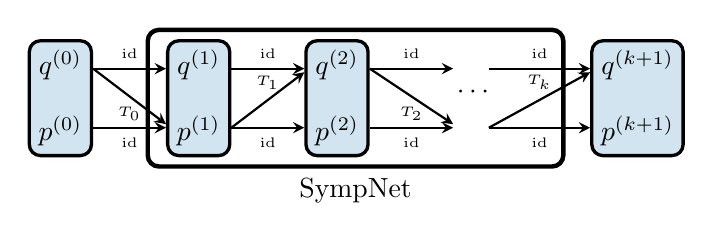
\begin{tikzpicture}[module/.style={draw, very thick, rounded corners, minimum width=4ex},
    ffnnmodule/.style={module, fill=mblue!20},
    arrow/.style={-stealth, thick, rounded corners},
]

\node[ffnnmodule, align=center] (qp0) {$q^{(0)}$\\\\$p^{(0)}$};
\node[ffnnmodule, right of=qp0, align=center, xshift=5ex] (qp1) {$q^{(1)}$ \\ \\ $p^{(1)}$};
\node[ffnnmodule, right of=qp1, align=center, xshift=5ex] (qp2) {$q^{(2)}$ \\ \\ $p^{(2)}$};
\node[right of=qp2, align=center, xshift=5ex] (dots) { \\ $\cdots$ \\ };
\node[right of=dots, ffnnmodule, align=center, xshift=7ex] (qpn) {$q^{(k+1)}$ \\ \\ $p^{(k+1)}$};

\coordinate[right of=qp0, xshift=1.5ex] (leftofqp1);
\coordinate[right of=dots] (rightofdots);

\node[fit=(leftofqp1)(qp1)(qp2)(dots)(rightofdots), draw, ultra thick, rounded corners, label=below:SympNet] (sympnet) {};

\draw[arrow] ($(qp0.east)!0.5!(qp0.north east)$) -- ($(qp1.west)!0.5!(qp1.north west)$) node[midway, above] {\tiny id};
\draw[arrow] ($(qp0.east)!0.5!(qp0.south east)$) -- ($(qp1.west)!0.5!(qp1.south west)$) node[midway, below] {\tiny id};

\draw[arrow] ($(qp1.east)!0.5!(qp1.north east)$) -- ($(qp2.west)!0.5!(qp2.north west)$) node[midway, above] {\tiny id};
\draw[arrow] ($(qp1.east)!0.5!(qp1.south east)$) -- ($(qp2.west)!0.5!(qp2.south west)$) node[midway, below] {\tiny id};

\draw[arrow] ($(qp2.east)!0.5!(qp2.north east)$) -- ([xshift=7ex] $(qp2.east)!0.5!(qp2.north east)$) node[midway, above] {\tiny id};
\draw[arrow] ($(qp2.east)!0.5!(qp2.south east)$) -- ([xshift=7ex] $(qp2.east)!0.5!(qp2.south east)$) node[midway, below] {\tiny id};

\draw[arrow] ([xshift=10ex] $(qp2.east)!0.5!(qp2.north east)$) -- ($(qpn.west)!0.5!(qpn.north west)$) node[midway, above] {\tiny id};
\draw[arrow] ([xshift=10ex] $(qp2.east)!0.5!(qp2.south east)$) -- ($(qpn.west)!0.5!(qpn.south west)$) node[midway, below] {\tiny id};
 
\draw[arrow] ($(qp0.east)!0.5!(qp0.north east)$) -- ([yshift=.3ex] $(qp1.west)!0.5!(qp1.south west)$) node[midway, below] {\tiny $T_0$};

\draw[arrow] ($(qp1.east)!0.5!(qp1.south east)$) -- ([yshift=-.3ex] $(qp2.west)!0.5!(qp2.north west)$) node[midway, above] {\tiny $T_1$};

\draw[arrow] ($(qp2.east)!0.5!(qp2.north east)$) -- ([yshift=.3ex, xshift=7ex] $(qp2.east)!0.5!(qp2.south east)$) node[midway, below] {\tiny $T_2$};

\draw[arrow] ([xshift=10ex] $(qp2.east)!0.5!(qp2.south east)$) -- ([yshift=-.3ex] $(qpn.west)!0.5!(qpn.north west)$) node[midway, above] {\tiny $T_k$};

\end{tikzpicture}

\end{document}